\def \CILKserialbaseline {4267}
\def \CILKblocksize {64}
\def \CILKnumtrials {1}
\def \CILKinputsize {1073741824}
\def \CILKtable {
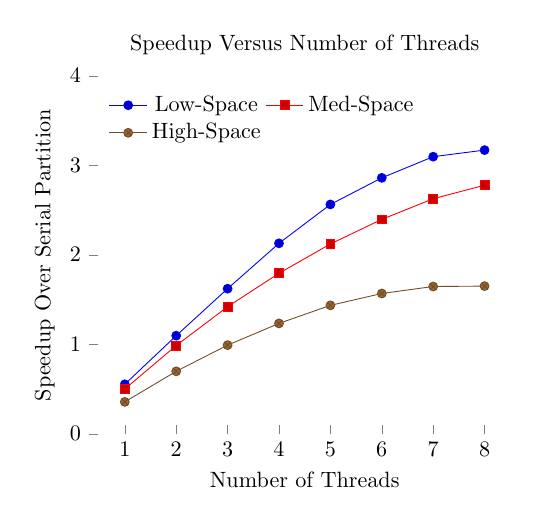
\begin{tikzpicture}[scale = .8]
\begin{axis}[
title={Speedup Versus Number of Threads},
xtick pos=left,
ytick pos=left,
legend style={draw=none},
axis line style = { draw = none },
legend pos= north west,
xtick = data,
xlabel={Number of Threads},
ylabel={Speedup Over Serial Partition},
ymax = 4,
legend columns = 2,
scatter/classes=%
{a={mark=o,draw=blue}}]
%% In-Place
\addplot coordinates {( 1, 0.552935) ( 2, 1.09607) ( 3, 1.6212) ( 4, 2.12818) ( 5, 2.56276) ( 6, 2.85992) ( 7, 3.09652) ( 8, 3.17013) };
%% In-Place Prefix-Sum
\addplot coordinates {( 1, 0.499766) ( 2, 0.985906) ( 3, 1.41949) ( 4, 1.79361) ( 5, 2.12078) ( 6, 2.39585) ( 7, 2.62585) ( 8, 2.77799) };
%% Out-of-Place
\addplot coordinates {( 1, 0.356118) ( 2, 0.697678) ( 3, 0.990253) ( 4, 1.23324) ( 5, 1.43477) ( 6, 1.5676) ( 7, 1.64558) ( 8, 1.65004) };
\legend{Low-Space, Med-Space, High-Space}
\end{axis}
\end{tikzpicture}
}
\def \CILKblocksizetwo {64}
\def \CILKnumtrialstwo {1}
\def \CILKnumcorestwo {8}
\def \CILKinputsizetwo {1073741824}
\def \CILKtabletwo {
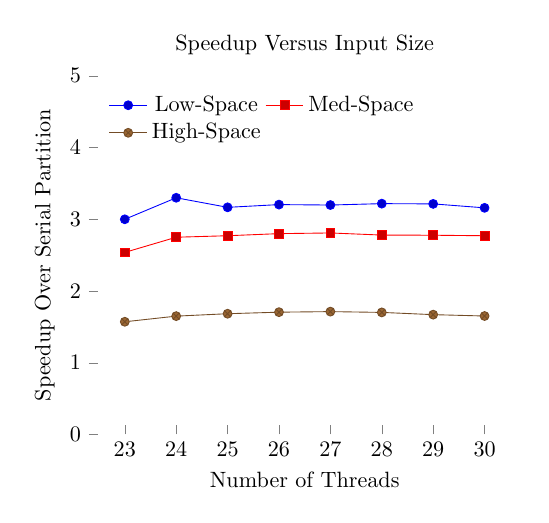
\begin{tikzpicture}[scale = .8]
\begin{axis}[
title={Speedup Versus Input Size},
xtick pos=left,
ytick pos=left,
legend style={draw=none},
axis line style = { draw = none },
legend pos= north west,
xtick = data,
xlabel={Number of Threads},
ylabel={Speedup Over Serial Partition},
ymax = 5,
ymin = 0,
legend columns = 2,
scatter/classes=%
{a={mark=o,draw=blue}}]
%% Serial Baseline
%% baselines in ms: \addplot coordinates {( 23, 33 ) ( 24, 66 ) ( 25, 133 ) ( 26, 266 ) ( 27, 531 ) ( 28, 1062 ) ( 29, 2125 ) ( 30, 4253 ) };
%% In-Place
\addplot coordinates {( 23, 3) ( 24, 3.3) ( 25, 3.16667) ( 26, 3.20482) ( 27, 3.1988) ( 28, 3.21818) ( 29, 3.21483) ( 30, 3.15973) };
%% In-Place Prefix-Sum
\addplot coordinates {( 23, 2.53846) ( 24, 2.75) ( 25, 2.77083) ( 26, 2.8) ( 27, 2.80952) ( 28, 2.7801) ( 29, 2.77778) ( 30, 2.77068) };
%% Out-of-Place
\addplot coordinates {( 23, 1.57143) ( 24, 1.65) ( 25, 1.68354) ( 26, 1.70513) ( 27, 1.7129) ( 28, 1.70192) ( 29, 1.6706) ( 30, 1.65165) };
\legend{Low-Space, Med-Space, High-Space}
\end{axis}
\end{tikzpicture}
}
